\documentclass[10pt, a4paper]{article}
\usepackage[utf8]{inputenc}
\usepackage{amsmath}
\usepackage{amssymb}
\usepackage{graphicx}
\usepackage{enumitem} % For custom list formatting
\usepackage{tikz} % For drawing simple diagrams
\usepackage{geometry} % To manage page margins
\usepackage{fancyhdr} % For header/footer control
\usepackage{xcolor} % For colorized solutions

% Set margins aggressively to maximize space and ensure 2-page fit
\geometry{
    a4paper,
    total={190mm,277mm},
    left=13mm,
    right=13mm,
    top=12mm,
    bottom=12mm,
}

\pagestyle{empty}

% Define solution color
\definecolor{answerblue}{rgb}{0.1, 0.3, 0.6}
\newcommand{\solution}[1]{\textbf{\color{answerblue}#1}}

\begin{document}
\begin{center}
    {\Large\textbf{Introduction to Graphs Worksheet}} \\
    {\large\textbf{SOLUTIONS}}
\end{center}

\hrule
\vspace{0.4cm}

\begin{enumerate}[label=\textbf{\arabic*.}]
    
    \item \textbf{Core Terminology}
    \vspace{0.1cm}
    \begin{enumerate}[label=(\alph*)]
        \item A graph where all edges have a numerical value associated with them is called a \solution{Weighted} graph.
        \vspace{0.3cm}
        \item The most space-efficient representation for a \textbf{sparse} graph in competitive programming is the \solution{Adjacency List}.
        \vspace{0.3cm}
        \item The number of edges connected to a specific vertex is called its \solution{Degree}.
        \vspace{0.2cm}
        \item A graph that contains a path that starts and ends at the same vertex is called \solution{Cyclic}.
        \vspace{0.3cm}
        \item A tree is a special type of graph that is undirected, connected, and \solution{Acyclic} (meaning it has no cycles).
    \end{enumerate}

    \vspace{0.4cm}
    \item \textbf{Graph Representation Efficiency}
    
    $V=10^5$, $E=10^6$.
    \vspace{0.2cm}
    \begin{enumerate}[label=(\alph*)]
        \item What is the approximate space complexity (in terms of $V$ and $E$) for an Adjacency Matrix representation? \solution{$O(V^2)$}
        \vspace{0.3cm}
        \item Calculate the approximate memory space required for the Adjacency Matrix (assuming one cell stores 4 bytes). \solution{$10^{10} \times 4$ Bytes} (40 Gigabytes)
        \vspace{0.3cm}
        \item What is the approximate space complexity for an Adjacency List representation? \solution{$O(V + E)$}
        \vspace{0.1cm}
        \item Which representation should you choose for this problem, and why? \newline
        \vspace{0.1cm}
        \solution{The \textbf{Adjacency List}. Because $V^2$ ($10^{10}$) is much larger than $V+E$ ($10^5 + 10^6$), the Adjacency List is far more memory efficient and is essential for avoiding a Memory Limit Exceeded (MLE) error.}
        \vspace{0.25cm}
    \end{enumerate}

    \vspace{0.4cm}
    \item \textbf{Analyzing a Sample Graph}
    
    \begin{center}
    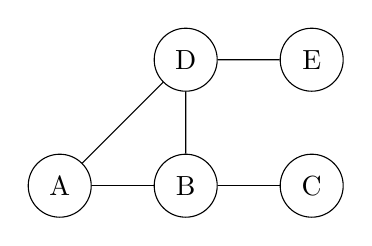
\begin{tikzpicture}[scale=0.8, every node/.style={draw,circle,minimum size=0.8cm,inner sep=0pt}]
        \node (A) at (0, 0) {A};
        \node (B) at (2, 0) {B};
        \node (C) at (4, 0) {C};
        \node (D) at (2, 2) {D};
        \node (E) at (4, 2) {E};
        
        \draw (A) -- (B);
        \draw (B) -- (C);
        \draw (A) -- (D);
        \draw (D) -- (E);
        \draw (B) -- (D);
    \end{tikzpicture}
    \end{center}
    
    \vspace{0.3cm}
    \begin{enumerate}[label=(\alph*)]
        \item What is the degree of vertex B? \solution{3 (connected to A, C, D)}
        \vspace{0.2cm}
        \item Write the Adjacency List for the graph above.
        \begin{itemize}[noitemsep, topsep=0pt, parsep=0pt, leftmargin=1.5cm]
            \item A: \solution{B, D}
            \item B: \solution{A, C, D}
            \item C: \solution{B}
            \item D: \solution{A, B, E}
            \item E: \solution{D}
        \end{itemize}
        \vspace{0.2cm}
        \item List one cycle in this graph (e.g., A-B-C-A). \solution{A-B-D-A} (or D-A-B-D)
    \end{enumerate}

    \newpage

    \item \textbf{Breadth-First Search (BFS) Traversal}

    Start at \textbf{A}.

    \vspace{0.2cm}
    \begin{enumerate}[label=(\alph*)]
        \item What is the order in which the vertices are \textbf{visited} (printed/processed)?
        \textbf{Start:} A \quad \solution{B, D, C, E}
        \vspace{0.3cm}
        \item What is the shortest distance (in number of edges) from A to C? \solution{2} (Path A $\to$ B $\to$ C)
        \vspace{0.3cm}
        \item What is the key advantage of using BFS for pathfinding in unweighted graphs? 
        \vspace{0.1cm}
        \solution{It guarantees finding the path with the \textbf{minimum number of edges} because it explores all vertices at distance $k$ before moving to vertices at distance $k+1$.}
    \end{enumerate}

    \vspace{0.4cm}
    \item \textbf{Depth-First Search (DFS) Traversal}

    Start at \textbf{A}. Neighbors visited alphabetically (A $\to$ B $\to$ D $\to$ E).

    \vspace{0.2cm}
    \begin{enumerate}[label=(\alph*)]
        \item What is the order in which the vertices are \textbf{visited} (printed/processed)?
        \textbf{Start:} A \quad \solution{B, C, D, E} (A $\to$ B $\to$ C. Backtrack. A $\to$ D $\to$ E. Finished.)
        \vspace{0.3cm}
        \item True or False: If you ran a DFS starting at A, you would eventually visit C. \solution{True}
        \vspace{0.3cm}
        \item What is a primary use case for DFS that BFS is not optimized for? \newline
        \vspace{0.3cm}
        \solution{\textbf{Cycle Detection}, \textbf{Topological Sort} (on DAGs), and finding \textbf{Connected Components}.}
    \end{enumerate}

    \vspace{0.4cm}
    \item \textbf{Algorithm Selection Challenge}

    \vspace{0.2cm}
    \begin{enumerate}[label=(\alph*)]

        \item \textbf{Scenario:} Determine if you can reach the final commit from the initial commit in a Git repository (a DAG).
        \begin{itemize}[noitemsep, topsep=0pt, parsep=0pt, leftmargin=1.5cm]
            \item \textbf{Algorithm:} \solution{DFS} (or BFS)
            \item \textbf{Reason:} \solution{Any traversal (DFS or BFS) can check simple reachability/connectivity in linear time $O(V+E)$.}
        \end{itemize}
        \vspace{0.3cm}

        \item \textbf{Scenario:} A delivery robot must find the route with the fewest intersections in an unweighted map.
        \begin{itemize}[noitemsep, topsep=0pt, parsep=0pt, leftmargin=1.5cm]
            \item \textbf{Algorithm:} \solution{BFS}
            \item \textbf{Reason:} \solution{The problem asks for the minimum number of edges (fewest intersections) in an unweighted graph, which is the definition of BFS's result.}
        \end{itemize}
        \vspace{0.3cm}

        \item \textbf{Scenario:} You need the shortest path between two cities when roads have varying distances (weights).
        \begin{itemize}[noitemsep, topsep=0pt, parsep=0pt, leftmargin=1.5cm]
            \item \textbf{Algorithm:} \solution{Neither} (Use Dijkstra's)
            \item \textbf{Reason:} \solution{The edges are \textbf{weighted}, so BFS cannot guarantee the shortest path. Dijkstra's Algorithm is required for shortest paths in weighted graphs (with non-negative weights).}
        \end{itemize}

    \end{enumerate}

\end{document}